\documentclass{article}
\usepackage{graphicx} 
\usepackage[backend=biber, natbib =true, style=apa]{biblatex}
\usepackage{multirow}
\usepackage[normalem]{ulem}
\useunder{\uline}{\ul}{}
\usepackage{geometry}                  
\usepackage{booktabs, multirow}        
\usepackage[referable]{threeparttablex}
\usepackage{float} 
\addbibresource{ref_RR_21dec.bib}
\usepackage{booktabs}
\usepackage{threeparttable}
\usepackage{tabularx}
\usepackage{ragged2e}
\usepackage{array}
\usepackage{placeins}


\title{Variation in Many-Analyst Projects: Harmful or Helpful? A Multiverse Approach to Address Different Sources of Variation \\ \small Research Report} 
\author{Loesje Ubbink (6077137) \\ Thesis Supervisor: Suzanne Hoogeveen \\ \\ \small Methodology and Statistics for the Behavioural, Biomedical and Social Sciences \\ \small Faculty of Social and Behavioural Sciences\\ \small Utrecht University \\ \\ \small Candidate Journal: Royal Society of Open Science \\ \small Candidate Journal: Advances in Methods and Practices in Psychological Science  \\ \\ FETC Registration Number: 25-2021 (accepted) \\ \\ Word Count: 2498}
\date{December 21, 2025}

\begin{document}

\maketitle
\newpage
\section*{Introduction}
Over recent years, it has become increasingly clear that the scientific community is facing a replication crisis \citep[e.g.,][]{forbes_supporting_2023}. A growing number of studies have reported difficulties reproducing previously published findings. This problem is often attributed to publication bias – the tendency to only publish significant results – and questionable research practices (QRPs). However, even studies aimed at removing the incentive for QRPs have painted a rather pessimistic picture of reproducible science \citep{auspurg_toward_2024}. Many-analyst studies, where multiple independent researchers answer the same research question using the same dataset, have shown considerable variation in analytic strategies and results \citep[e.g.,][]{silberzahn_many_2018, bastiaansen_time_2020,breznau_observing_2022,hoogeveen_many-analysts_2023, gould_same_2025, kowall_marital_2025}. Reported effect sizes often vary from negative to positive, and from significant to non-significant, all within the same study. This means that there is not only considerable variation in the results but also in the substantive conclusions drawn from them. At first glance, this seems an immediate threat to the reproducibility of science. In an ideal world, one might expect that a single dataset should yield a single, `true' answer, raising the question whether outcome variation should always be interpreted as problematic.

However, interpreting this variation without understanding its origins may not be that straightforward. A frequently raised criticism of many-analyst projects is that the posed research questions are often too vague, leaving analysts uncertain about how to proceed with data analysis and which variables should be included in their statistical models \citep{kummerfeld_one_2023, hoogeveen_many-analysts_2023-1}. This uncertainty is particularly problematic in situations where researchers are implicitly interested in finding causal relationships, which is often the case in many-analyst projects \citep{del_giudice_travelers_2021, bulbulia_workflow_2023, rohrer_what_2025}. In this context, including different confounders may correspond to different causal assumptions and thus different – potentially opposing – estimated effects. Therefore, when analysts select different variables, they may in fact be answering different questions \citep{simonsohn_specification_2015}. From this perspective, outcome variation may indicate meaningful substantive differences rather than problematic analytical noise. On the other hand, if the outcome variation stems from arbitrary, equally justifiable decisions whose options do not reflect different substantive meanings, this may be considered more problematic \citep{del_giudice_travelers_2021}. 

\subsection*{The AB-framework}
For better interpretation of outcome variation in many-analyst projects, \citet{auspurg_toward_2024} have introduced a theoretical framework (hereafter referred to as the AB-framework) to distinguish between three different sources of variation, two of which are considered `harmful' and one `helpful' (see Table~\ref{tab:AB_framework}). 

\begin{table}[H]
\centering
\caption{Sources of variation according to \citet{auspurg_toward_2024}}
\label{tab:AB_framework}
\begin{threeparttable}
\footnotesize
\setlength{\tabcolsep}{10pt}
\renewcommand{\arraystretch}{1.2}

\begin{tabular}{
>{\RaggedRight\arraybackslash}p{7.2cm}
>{\RaggedRight\arraybackslash}p{7.2cm}
}
\toprule
\textbf{Harmful} & \textbf{Helpful} \\
\midrule

(a) Model uncertainty, including subjective analytical choices in data handling (e.g., missing data decisions, weighting etc.) and the selection of statistical models with different assumptions

\vspace{0.4em}
(b) Coding errors
&
(c) Substantively meaningful variation arising from different definitions of dependent, independent, and confounding variables, as well as differences in target populations (e.g., exclusion criteria or changes over time) \\

\bottomrule
\end{tabular}

\end{threeparttable}
\end{table}

First, outcome variation may arise from model uncertainty (a), for example in missing-data imputation or modelling assumptions, reflecting ambiguity about the correct approach to estimate the parameter of interest and its underlying data-generating process. For example, if different imputation strategies (e.g., mean versus multiple imputation) result in different mean effect sizes, while the underlying observed data remain the same, this would imply that the outcome depends on an arbitrary analytic choice rather than on the data themselves. Secondly, outcome variation may be the result of sloppiness or hidden coding errors (b) made by the analysts. Both sources can be considered harmful, as they can introduce undesirable uncertainty into scientific analyses, making conclusions less credible.

In contrast, the third source concerns analytical choices that provide information about substantive variation that actually exists in the population (c). As mentioned earlier, selecting different target populations or confounders can lead to slightly different questions being answered. For example, if analyst X uses the full dataset, while analyst Y analyses only the men in that same dataset, X might find no effect in the general population, while Y finds that there is a male-specific positive effect. Given that the two analysts answered different questions, this source can be considered as helpful for the advancement of theories. By taking a closer look at the decisions made by analysts and the implications thereof, the AB-framework provides tools to interpret outcome variation in many-analyst projects.

\subsection*{Identifying sources of variation in many-analyst projects}
Although several many-analyst studies have aimed to identify the sources of outcome variation, so far no consensus has been reached \citep[e.g.,][]{silberzahn_many_2018, bastiaansen_time_2020,breznau_observing_2022,hoogeveen_many-analysts_2023, gould_same_2025, kowall_marital_2025}. For example, \citet{hoogeveen_many-analysts_2023} found that the operationalisations of variables, rather than model choice,  influenced the results the most. In contrast, \citet{gould_same_2025} showed that neither variation in variable selection nor model structure meaningfully predicted variability, but did not explicitly name another explanation source of variation. A similar pattern was found by \citet{kowall_marital_2025}, where data structure (cross-sectional versus longitudinal), rather than model or variable choice, likely had the largest impact on the results. Different studies thus highlight different sources of variation. 

Given the wide variety of topics, designs, and variables across projects, it may be unrealistic to expect a single, fixed set of explanatory factors that applies to all studies. However, even identifying a study-specific source of variation might not be possible based on many-analyst studies alone. A key limitation of these projects is that the involved analysts make decisions in an uncontrolled way \citep{kummerfeld_one_2023}. This leads to the problem of sparse data, where little data is generally available for each individual decision, as unique combinations of choices are often chosen only once. This sparsity makes it difficult to properly disentangle individual sources of variation and provide systematic quantitative evidence of their relative influence. Consequently, solely looking at analytical decisions in many-analyst projects may not provide enough information to interpret outcome variation with the AB-framework.

\subsection*{Multiverse analysis}
One approach to addressing the problem of data sparseness is multiverse analysis \citep[e.g.,][]{steegen_increasing_2016, hoogeveen_many-analysts_2023-1}. First, this method identifies all reasonable decisions, each with a specific number of options, and systematically combines them into a decision space \citep{liu_approximation_2023}. Since not all combinations may yield possible analyses, the set of valid analysis paths (universes) is always smaller than or equal to the full product. Then, results are reported across all valid universes. This way, multiverse analysis allows for the exploration of the entire decision space, rather than just a subset of choices made by analysts. As a result, substantially more data are available for each decision, enabling quantification of their specific impact on the results.

Although multiverse analysis seems a promising way of systematically evaluating the sensitivity of decisions, one of its limitations is that the decision space is often defined by a single researcher \citep{simonsohn_specification_2015}. Consequently, some reasonable analysis paths may be overlooked. However, by basing the multiverse analysis on an existing many-analyst project, this problem can be solved. The decision space will then be determined by the ``wisdom of the crowd” and represent realistic research choices \citep{auspurg_toward_2024}. 

Another limitation is that different universes with contradicting substantial implications may be included within the same multiverse. \citet{del_giudice_travelers_2021} argue that as a solution, a multiverse should only include truly arbitrary, but not theoretically meaningful decisions, as the latter may lead to misleading results. However, by including both types of decisions and subsequently classifying them with the AB-framework, results that might otherwise be considered misleading could instead be interpreted in a meaningful way.

\subsection*{Present study}
To assess the current state of the replication crisis using many-analyst projects, it is highly relevant to identify the most prominent sources of variation and their implications based on the AB-framework. Due to the descriptive nature of many-analyst studies, no consensus has yet been reached about what factors drive variability in the results, leading to the research question: \emph{What is the relative contribution of harmful versus helpful analytical decisions in many-analyst projects to outcome variation when they are systematically evaluated in a multiverse?}

Aiming to gain quantitative evidence of the relative influence of different sources of variation, the present study will conduct a multiverse analysis based on the many-analyst project by \citet{kowall_marital_2025}, where 16 teams analysed whether marital status (cohabiting married versus never married) predicts cardiovascular disease. This was chosen as a case study, because there was a large variety of both harmful and helpful decisions, providing a rich decision space to evaluate the impact of a wide range of different decisions. The decision space consists of six analytical decisions: handling missing data, choice of exclusion criteria, statistical model and definitions of dependent variables, confounders and target population. Before running the analysis, these decisions are classified as harmful/helpful using the AB-framework. The multiverse analysis is largely based on sampling and approximation methods proposed by \citet{liu_approximation_2023}, where the decision space is sampled to immediately calculate the mean effect and decision sensitivity. Lastly, a specification curve will be plotted to visualise how the outcomes relate to different analysis paths. For more details, see the Methods section.

\section*{Methods}
\subsection*{Ethics}
Ethical approval was granted by the Ethics Review Board of the Faculty of Social and Behavioural Sciences of Utrecht University. 

\subsection*{Data} 
Although the original teams’ results are not analysed directly, the multiverse is applied to the same data they analysed in \citet{kowall_marital_2025}, namely the Survey of Health, Ageing and Retirement in Europe (SHARE). This is a freely available (after registration) panel study conducted in 28 European countries. Consistent with the original study, waves 1-7 are used. As some analysts used the imputed SHARE datasets, these are also used here.

All variables needed for the construction of the decision space (e.g., dependent, independent, confounders, exclusion) are selected from different relevant datasets that are available per wave. Then, one cleaned dataset is created per wave, where the selected variables are linked through an ID variable. 

\begin{table}[htbp]
\centering
\caption{Identification and classification of analytical decisions and their options from \citet{kowall_marital_2025} that will be used for the present multiverse.}
\label{tab:decision_space}
\begin{threeparttable}
\footnotesize
\setlength{\tabcolsep}{6pt}
\renewcommand{\arraystretch}{1.25}

\begin{tabularx}{\textwidth}{
>{\RaggedRight\arraybackslash}p{3.2cm}
>{\RaggedRight\arraybackslash}p{6.2cm}
>{\RaggedRight\arraybackslash}X
}
\toprule
\textbf{Decision} & \textbf{Options} & \textbf{Notes / Deviations from original} \\
\midrule

\multicolumn{2}{l}{\textbf{Harmful sources of variation}} \\
\midrule

Missing data &
Complete cases (16) \newline
Imputed SHARE data (3) \newline
``No information'' (1)
&
For complete cases, listwise deletion is applied. Occasionally, the imputed dataset provided by SHARE is used. One team replaced missing values by ``no information'' to prevent listwise deletion. \\

\addlinespace

Model type &
Cox proportional hazards model (6) \newline
Logistic regression (5) \newline
Log-binomial model (2) \newline
Mixed-effects logistic regression (1) \newline
Discrete-time mixed-effects model (1) \newline
Generalised estimating equations (1)
&
Originally, different effect sizes were reported. For comparability, this multiverse analysis reports odds ratios only. \\

\addlinespace

\multicolumn{3}{l}{\textbf{Helpful sources of variation}} \\
\midrule

Data structure &
Strictly longitudinal (10) \newline
Longitudinal, wave 1 as only baseline (3) \newline
Strictly or partly cross-sectional (6)
&
The cleaned datasets for each wave are combined in different ways, depending on the selected option. \\
\addlinespace

Exclusion criteria &
Subjects married before 18 \newline
Subjects from Israel \newline
Subjects under 55 at recruitment \newline
Subjects born after 1954
&
Because the original article did not specify whether combinations were used, a maximum of one exclusion criterion per universe was applied. \\

\addlinespace
\addlinespace
Dependent variables &
Heart attack / stroke ever (16) \newline
Age at heart attack / stroke (9) \newline
Heart attack / stroke since last interview (7) \newline
Main cause of death: heart attack / stroke (5)
&
Seven combinations of the four dependent variables were created. Although other combinations are possible, these are assumed to be less realistic and therefore not included in the decision space. \\

\addlinespace

Confounders &
Age (12) \newline
Sex (12) \newline
Country (7) \newline
Smoking (6) \newline
Education (4) \newline
Physical activity (4) \newline
No confounders (2)
&
Only confounders used by at least four analysts, except `no confounders', were included to ensure feasibility. \\

\bottomrule
\end{tabularx}

\begin{tablenotes}[flushleft]
\footnotesize
\item \textit{Note}. Numbers in parentheses indicate how often each option was selected across analytical teams.
\item \textit{Note}. For the independent variable (IV), all teams but two used “cohabiting married” (CM). The exceptions also included registered partnership, and married living apart. However, since the original research question only focused on CM, this is the only variable used as IV.

\end{tablenotes}

\end{threeparttable}
\end{table}

\subsection*{Definition of decision space} 
To define the decision space, all options of six different decisions made by the teams in Kowall et al. (2025) are identified based on information provided in the original publication (see Table~\ref{tab:decision_space}). When systematically combining all options across decisions, the decision space consists of 193.536 universes – before removing invalid research paths.

\subsection*{Classifying sources of variation using the AB-framework}
Before running the analyses, the selected decisions are classified using the AB-framework. Decisions regarding missing data and statistical model choice are considered harmful. Decisions regarding the operationalisation of the dependent variable and the selection of confounders and exclusion criteria are considered helpful. Additionally, because the framework classifies variations over time as `different target populations’, which are meaningful, the data structure is classified as helpful. Table ~\ref{tab:decision_space} also includes the classification of decisions.

\begin{figure}[H]
    \centering
    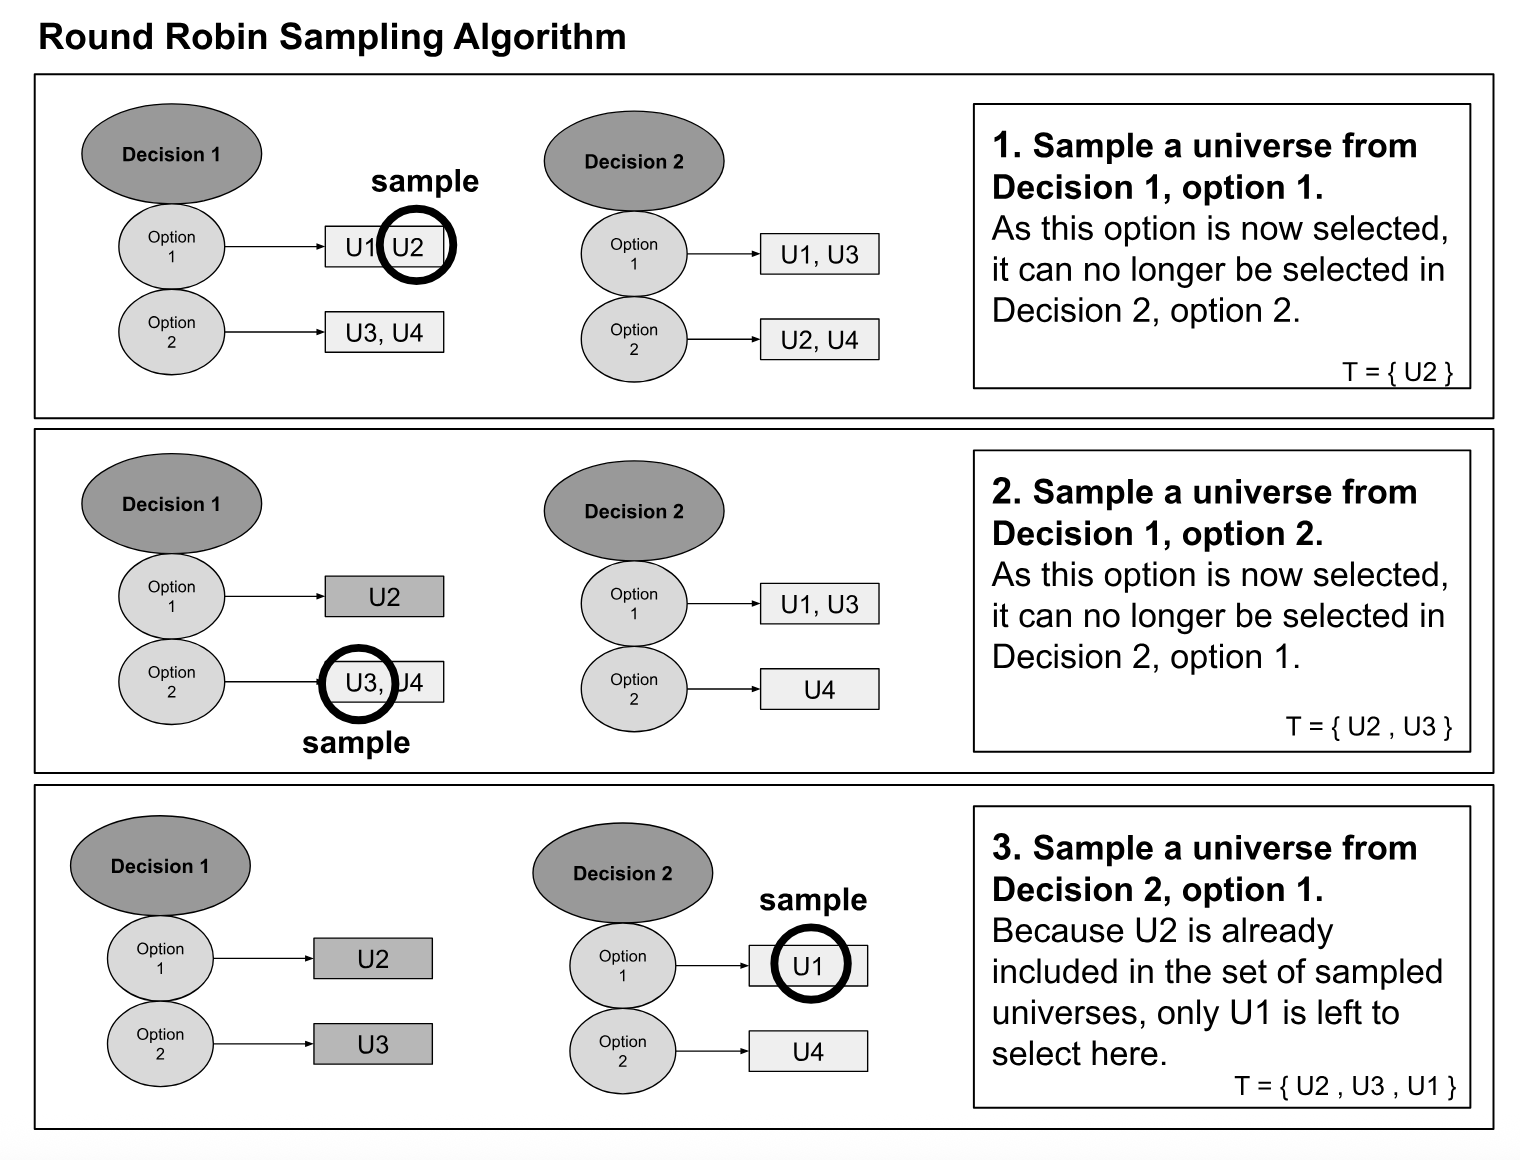
\includegraphics[width=1\linewidth]{round_robin_schematic.png}
    \caption{Schematic overview of Round Robin sampling algorithm. U: universe; T: the set of selected universes. Figure was created by the author for this research report.}
    \label{fig:round_robin}
\end{figure}

\subsection*{Round Robin sampling}
Because the number of reasonable universes grows exponentially with the number of decisions and their options, the computational cost of multiverse analyses increases rapidly. To solve this problem, \citet{liu_approximation_2023} have proposed sampling universes one by one. By directly calculating their outcomes and decision sensitivities, it is possible to approximate multiverse results without having to explore the full decision space. They evaluated various algorithms and found that Round Robin sampling was one of the most effective methods. Therefore, this method will be applied in the present study. 

Round Robin sampling aims to represent each decision option in the multiverse at least once. The algorithm iteratively goes over all decisions and their options and samples one universe at each stage. The sampling is done without replacement, to make sure each sampled universe is included at most once. For a visual example of how the algorithm works, see Figure~\ref{fig:round_robin}. 

When defining the number of sampled universes, it is important to make sure enough data is available for every option to quantify the decision sensitivity. The operationalisations of the dependent variable and the confounders have the most options (7 and 128, respectively). Assuming a sample size of at least 30 outcomes/universes per option (or more if that is feasible computationally and within the time scope of this project), this would result in $128 \times 30 = 3840$ sampled universes in total.

\subsection*{Decision sensitivity}
So far, the robustness of multiverse outcomes has often been assessed using specification curve analysis (SCA). In this type of analysis, each universe is plotted against its associated estimated effect size \citep{simonsohn_specification_2015}. However, as this only provides information about the robustness of the results, but not the decision sensitivity, it will only be used as a visual aid to inspect if the full outcome distribution is robust to different analytic strategies.

More recently, \citet{liu_approximation_2023} have proposed using the K-samples Anderson-Darling test (AD-test) to quantify not only the robustness of the results, but also the decision sensitivity – the extent to which different options within each analytical decision lead to different outcomes. For each option, an effect size distribution is constructed, consisting of the results from all universes containing that option (see Figure~\ref{fig:sim_DV_dist} for an example). This means that within each outcome distribution the option of one specific decision remains constant, while other analytical decisions and their options vary. Next, the AD test is used to test whether the outcome distributions of the different options within the same decision originate from the same underlying distribution. If this null hypothesis is rejected, the decision in question is classified as `sensitive'.

Given that there are 128 confounder options, consisting of combinations of 7 variables, it is uncertain whether the AD test will perform well. Should this not be the case, the confounders will be analysed in a slightly different way, namely by categorizing for each option whether or not it is included in the universe, resulting in two outcome distributions per option (included/excluded). In the case of the confounders, this would mean that there would be only 14 options instead of 128. A Kolmogorov-Smirnov (K-S) test, similar to the AD test but with two samples, will then be used to quantify whether the two outcome distributions originate from the same underlying distribution.

\subsection*{Bootstrapped estimates and sensitivity}
Because only a subset of the full multiverse is used, similar to \citet{liu_approximation_2023}, bootstrapping is used to obtain 95\%-confidence intervals (CI) around the resampled mean outcome estimate and the decision sensitivities.

\subsection*{Technical specifications}
All data are analysed using R, with packages tidyverse, ggalluvial, multiverse, lme4, survival, geepack, kSamples and dgof \citep{wickham_welcome_2019,brunson_ggalluvial_2020,sarma_multiverse_2021,masur_specr_2020,bates_fitting_2015,therneau__a_2024,halekoh_r_2006, scholz_ksamples_2019,arnold_dgof_2011, r_core_team_r_2024}. 

\newpage
\section*{Preliminary results}
Figure~\ref{fig:sim_DV_dist} shows simulated example distributions of outcomes from the universes across options of `dependent variable operationalisations', 1-5 were generated from a normal distribution, and 6-7 from a beta-distribution. Given that not all outcome distributions have the same underlying distribution, the AD-test will  classified this decision as `sensitive'. Because this is a substantially meaningful decision, this would mean that finding variation in the effect sizes may not be that problematic for the reproducibility of science. 

\begin{figure}[H]
    \centering
    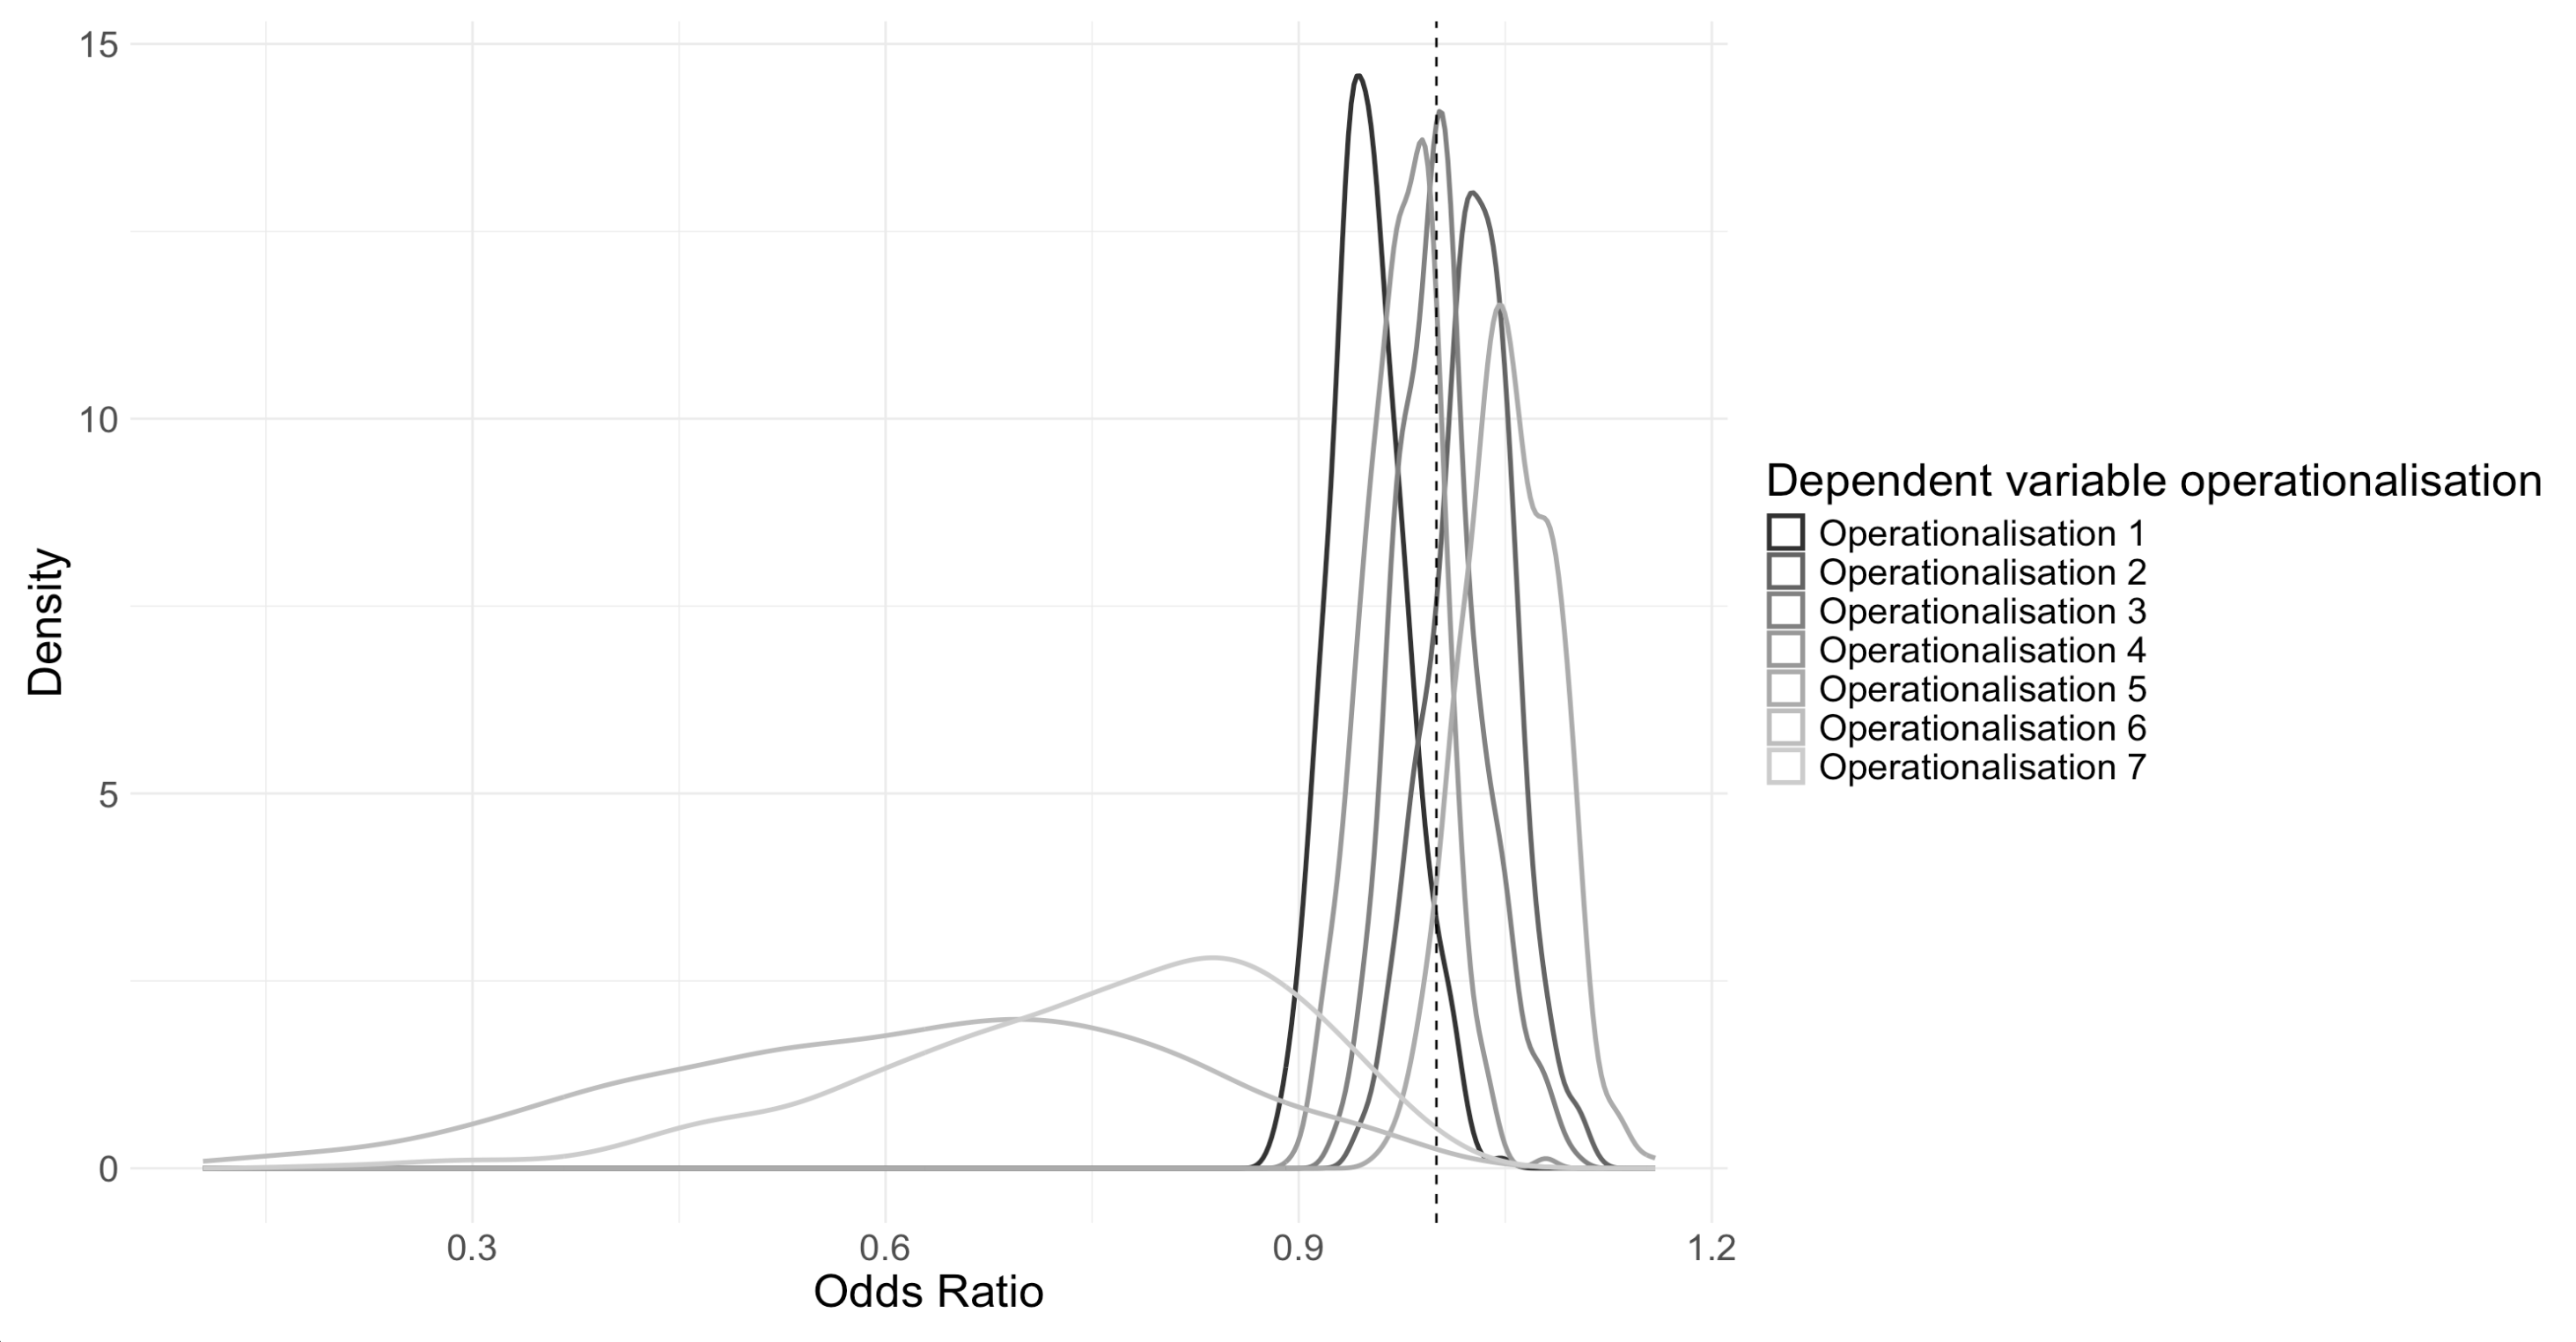
\includegraphics[width=1\linewidth]{simulated_OR_density.png}
    \caption{Simulated effect size distributions for the universes across all options of the decision `dependent variable operationalisation'.}
    \label{fig:sim_DV_dist}
\end{figure}

\newpage
\printbibliography[title={References}]


\end{document}